% ---------------------------------------------------
% ----- Introduction of the template
% ----- for Bachelor-, Master thesis and class papers
% ---------------------------------------------------
%  Created by C. Müller-Birn on 2012-08-17, CC-BY-SA 3.0.
%  Last upadte: C. Müller-Birn 2015-11-27 
%  Freie Universität Berlin, Institute of Computer Science, Human Centered Computing. 
%
\chapter{Thematic Introduction and Motivation}
\label{chap:introduction}

With the surge of the application of machine learning (ML) systems in our daily life there is an increasing demand to make operation and results of these systems interpretable for people with different backgrounds (ML experts, non-technical experts etc.). Considering that even the developers sometimes struggle to understand the reasoning and deductions of their own systems \cite{DeepPhenomena}, it is easy to imagine that the general public has a hard time understanding the capabilities and shortcomings of machine learning.

\section{Project IKON}

One project which operates in the cross section between machine learning and a non-technical target group is project \textit{IKON}. It tries to explore potentials for knowledge transfer activities at a research museum and was started in cooperation with the German Natural History Museum in Berlin which houses more than 300 scientists, PhD students and other staff \cite{Team2018}. With that size of scientific staff the institution is a global player in research on evolution and biodiversity \cite{IntroducingMuseumFur}. Despite its importance in the research landscape, the museum is challenged with a lack of shared knowledge across working groups and organizational structures such as departments\cite{benjamin_understanding_2019}. In interviews researchers from the project were able to trace these problems back to the very intricate and complex layout of rooms and halls in the building which was originally constructed in 1810 \cite{140JahreAltes2018}. In order to mitigate this problem \autoref{pic:IKON-clusterview} shows one of the main deliverables of IKON - a ML-driven data visualization which follows the path of knowledge at this research museum from its creation in projects over knowledge transfer activities, where multiple projects exchange their findings, to the final target group. Potentials for knowledge exchange are made explicit by visualizing projects not in the organizational hierarchy of the museum, but instead in semantic relation to each other. This approach has become evident from qualitative work done by the project researchers \cite{benjamin_understanding_2019}. Therefore, I have developed a topic modeling process consisting of four major components, as seen in \autoref{pic:general_topic_extraction_pipeline}. In the following section, I discuss the basic principles of such a pipeline, before moving on to the specific challenge of interpretability in this context.

\begin{figure}[htpb!]
	\centering
	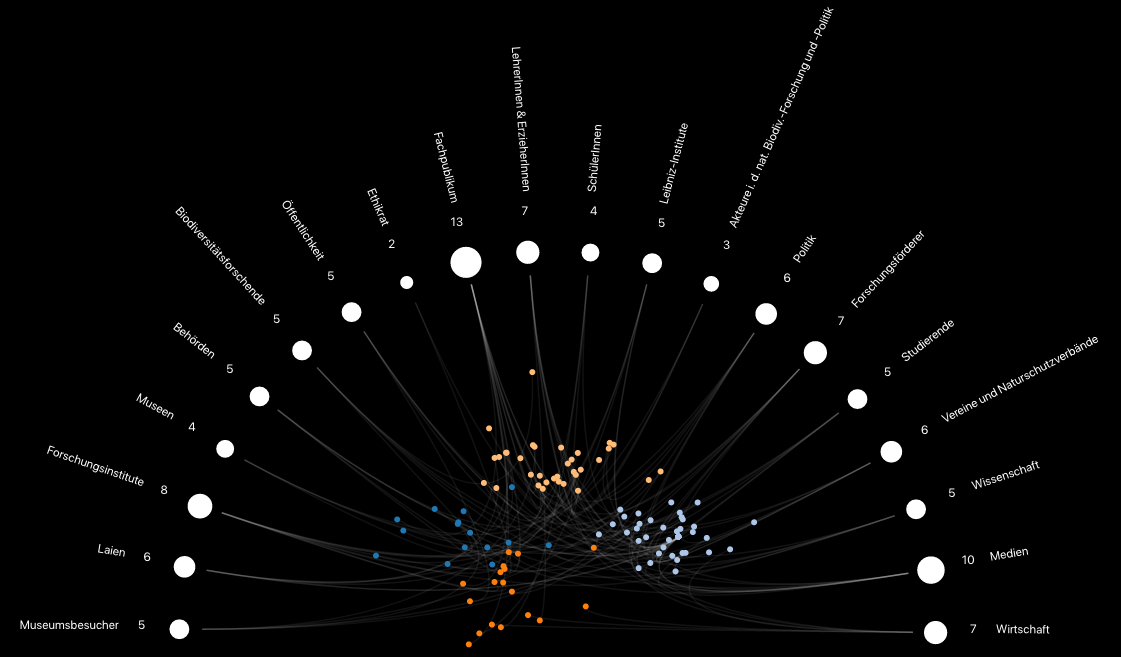
\includegraphics[width=400px]{../chapters/introduction/graphics/ikon-clusterview}
	\caption{\label{pic:IKON-clusterview} Screenshot of the cluster view of the IKON visualization}
\end{figure}

\section{Topic modeling}

% Define block styles
\tikzstyle{decision} = [diamond, draw, fill=blue!20, 
text width=4.5em, text badly centered, node distance=3cm, inner sep=0pt]
\tikzstyle{block} = [rectangle, draw, fill=blue!20, 
text width=6.5em, text centered, rounded corners, minimum height=4em]
\tikzstyle{line} = [draw, -latex']
\tikzstyle{cloud} = [draw, ellipse,fill=red!20, node distance=3cm,
minimum height=2em]
\usetikzlibrary{decorations.text}

\begin{figure}[htpb!]
	\centering
	\begin{tikzpicture}[node distance = 4cm, auto]
	% Place nodes
	\node [block] (emb) {Document embedding};
	%\node [cloud, left of=emb] (expert) {expert};
	%\node [cloud, right of=emb] (system) {system};
	\node [block, right of=emb] (topic) {Topic extraction};
	\node [block, right of=topic, above of=topic] (cluster) {Classification of documents};
	\node [block, right of=topic, below of=topic] (2D) {Reduction into 2D};
	% Draw edges
	\path [line] (emb) -- (topic);
	\path [line] (topic) -- (cluster);
	\path [line] (topic) -- (2D);
	%\path [line] (identify) -- (evaluate);
	%\path [line] (update) |- (identify);
	%\path [line,dashed] (system) |- (evaluate);
	\end{tikzpicture}
	\caption{\label{pic:general_topic_extraction_pipeline} Components of a general topic extraction pipeline}
\end{figure}

A generic topic modeling pipeline consists of four steps: 
\begin{enumerate}
	\item Document embedding
	\item Topic extraction
	\item Classification of documents
	\item Reduction into 2D
\end{enumerate}

Given an unlabeled corpus $C = \{D_1, ..., D_n\}$ consisting of $n$ documents $D_i = (t_1, ..., t_m)$, which in turn consists of a sequence of $m$ strings, also called tokens or words, the document embedding step assigns to each document a vector $v_D \in \mathbb{R}^e, e \in \mathbb{N}^+$. Semantically similar documents should also be closer in the embedded vector space with respect to a given distance measure than documents which are semantically not related. Therefore this step transforms a corpus into a matrix $(v_1, ..., v_n) \in \mathbb{R}^{e \times n}$.

Consuming the output from the previous step the topic extraction tries to uncover $k$ latent structures. We call these structures \textit{topics}. Mathematically speaking a topic is a probability distribution over a fixed set of input features. \cite{liuOverviewTopicModeling2016} These features can correspond to tokens, as it is the case in the later discussed Tfidf-BOW embedding, but this does not have to be the case. Therefore this step transforms the corpus from the embedding space of dimensionality $e \times n$, where each document is described as linear combination of features, to the latent space of dimensionality $k \times n$, where each document is described as a linear combination of latent topics. Since most often $k < e$ holds true, this can also be seen as a form of dimensionality reduction, which is again a form of feature extraction.

Using the document vectors in the latent space each document is assigned a label. This may happen in a supervised way if there are labels available for training purposes, but in most cases an unsupervised classification, also known as clustering, is used to group the documents.

The last step is formally not part of the topic modeling itself, but if the use case demands a way to visualize the high dimensional distribution of documents in the latent space, another dimensionality reduction is used to project the documents to 2D. Since this is the case I include it in the process as well.

Each component in \autoref{pic:general_topic_extraction_pipeline} comes with its own set of parameters which influence the results generated by the pipeline. Therefore the researchers from project IKON hypothesize, based in first interviews and conceptual work, that the museum's staff, as non-technical experts without knowledge of the capabilities and shortcomings of the models used in topic modeling, will have a hard time interpreting and understanding the output generated by the pipeline. 

In order to lay the groundwork for this thesis and understand the challenges which scientists face while interacting with the visualization I carried out an exploratory workshop with the researchers from project \textit{IKON}. In the beginning I asked them which kind of hardships they, based on their past experiences and interviews, hypothesize during the interaction between user and visualization. Followed by an explanation of \autoref{pic:general_topic_extraction_pipeline} we discussed how these challenges may correlate with specific components and steps of the topic extraction pipeline. Following a description of the key questions each question was categorized according to the pipeline step, as seen in \autoref{tab:overview_viz_questions}, which may contribute information in order to support the user in answering his question.

\begin{table}
	\centering
	\begin{tabular}{ c | c }
		\hline 
		Question & Applicable pipeline component \\ \hline
		How does the research landscape look like \\ and on what kind of topics are prominent? & Topic Extraction \\ \hline
		What does a cluster mean? & Classification \\ \hline
		What does the distance between \\ clusters/projects mean? & Topic Extraction / Reduction into 2D \\ \hline
		How similar are two projects/clusters? & Topic Extraction \\
		\hline
	\end{tabular}
	\caption{\label{tab:overview_viz_questions} Table showing the sourced questions and the pipeline step which could provide an answer}
\end{table} 

\section{Interpretability}

Due to the long-standing issue of visualizing the museum research projects, there was already an existing NLP pipeline in project IKON which I had implemented as a proof-of-concept.. However, due to the concerns discussed above, the researchers became focused on the challenge of interpretability, which I discuss in this section. 
In the same workshop we also developed a way of structuring commonly used terminology in the field of explainability/interpretability research, where terms explainability and interpretability are commonly used as synonyms. Our notion builds upon the findings of Lipton, who suggested that, interpretability as a term is an ill-defined objective \cite{liptonMythosModelInterpretability2016a} for research and development in ML algorithms since there is no widely agreed upon definition of it. This leads to a very fragmented nature of the field. Furthermore Miller et al. \cite{millerExplainableAIBeware2017} support this point by conducting a literature study and uncovering that interpretability research is rarely influenced by insights from the humanities, especially connected fields such as explainability or causality research.

Therefore the researchers from project IKON hypothesize that the context in which interpretation is performed is essential to the outcome of the interpretative process. In this discussion the term 'context' considers the situational context of the interaction between user and system as well as the historical experiences of the user. The IKON researchers therefore proposed \footnote{Forthcoming publication.} a relational model in which users posses a set of \textit{a priori} preferred explanation strategies (e.g. comparing two entities) given the context of the interaction and their previous experiences. As a consequence of having this preferred set, they only consider a specific subset of all possible types of explanations as valid. Interpretability techniques on the other hand are conditioned in regard to an algorithmic system, e.g. a specific model or class of models. These techniques can be described by algorithms and deliver concrete explanations given a model and a model output. Therefore an interpretability technique serves as the missing link between high-level explanation strategies, an algorithmic system and explanations.
The algorithmic system upon which these interpretability techniques are build on was implemented as a proof-of-concept by me before the start of this thesis. Building the pipeline brought up serious concerns and uncertainty concerning the meaningfulness of approaches such as parameter manipulation or choosing between algorithms for dimensionality reduction \cite{benjaminTransparencyMediationMeaning2018} in our use case. Therefore I will explore the space of alternative methods. I developed a working plan for my thesis, which I will outline in the following section.
 

\begin{figure}[htpb!]
	\centering
	\begin{tikzpicture}[node distance = 6cm, auto]
	% Place nodes
	\node [block] (strat) {Explanation strategy};
	\node [block, right of=strat] (expl) {Explanation};
	\node [block, below of=strat] (alg) {Algorithmic system};
	\node [block, below of=expl] (int) {Interpretability technique};
	% Draw edges
	\path [line,dashed,
	postaction={decorate},
	decoration={text along path,
		text=requires,
		text align={left indent={0.2\dimexpr\pgfdecoratedpathlength\relax}}
	}] 
	(strat) -- (expl);
	
	\path [line,
	postaction={decorate},
	decoration={text along path,
		text=instantiates,
		text align={left indent={0.2\dimexpr\pgfdecoratedpathlength\relax}}
	}] 
	(int) -- (expl);
	
	\path [line,
	postaction={decorate},
	decoration={text along path,
		text=uses,
		text align={left indent={0.2\dimexpr\pgfdecoratedpathlength\relax}}
	}]
	(strat) -- (int);
	
	\path [line,
	postaction={decorate},
	decoration={text along path,
		text=conditions,
		text align={left indent={0.2\dimexpr\pgfdecoratedpathlength\relax}}
	}] 
	(alg) -- (int);
	\end{tikzpicture}
	\caption{\label{pic:interpretability_relational} Proposed model by the researchers showing the interplay of explanation strategies, interpretability techniques and explanations}
\end{figure}

\section{Working plan}
In order to research which interpretability techniques could be applied in project IKON, I conducted the following three steps:

\begin{enumerate}
	\item Since I as a developer did not possess an exhaustive list of techniques to enhance interpretability for unsupervised NLP models exist, a thorough and reproducible literature analysis on the status of XAI research in the field of NLP according to Petersen et al. \cite{petersenSystematicMappingStudies} is going to be conducted. This method should result in a number of papers which are, according to the process, good representatives of the literature base and therefore also of current research efforts. A quantitative analysis of these papers should summarize occurring XAI methods and categorize them according to an applicable categorization. 
	
	\item The currently existing topic extraction pipeline can be generalized into the following four components: document embedding, dimensionality reduction into a topic space, clustering and another dimensionality reduction into 2D. Based on the results of the previous step for each component either a directly applicable method (e.g. a clustering algorithm) from a paper or a model which supports most collected methods (e.g. a neural network for document embedding) is chosen and implemented. Since the new pipeline should capture at least as much information as the old one, each component will be quantitatively accessed according to applicable measures e.g. (\cite{roderExploringSpaceTopic2015a}). This is necessary to ensure that one is actually interpreting existing and captured semantic relations and not random artifacts generated by the various methods.
	
	\item A full user study would normally be necessary to assess how the implemented methods may support a non-technical expert in interpreting the results of the pipeline, but in order to keep the volume of this thesis in a feasible frame I will resort to a cognitive walkthrough from the point of view of a researcher from the national natural history museum.
	Since ensuring robustness in such qualitative tests is always a concern, information from previous interviews with domain experts from the museum will be used to derive meaningful tasks. The walkthrough should show how the user interacts with the implemented interpretability techniques.
\end{enumerate}

